\documentclass[11pt,a4paper]{article}
\usepackage[utf8]{inputenc}
\usepackage[english,catalan]{babel}
\usepackage[gen]{eurosym}
\usepackage[pdftex, pdfborderstyle={/S/U/W 0}]{hyperref} % this disables the boxes around links
\usepackage{longtable}
\usepackage[pdftex]{graphicx}

\usepackage{listings}
\usepackage{color}

\definecolor{dkgreen}{rgb}{0,0.6,0}
\definecolor{gray}{rgb}{0.5,0.5,0.5}
\definecolor{mauve}{rgb}{0.58,0,0.82}

\lstset{frame=tb,
  language=Java,
  aboveskip=3mm,
  belowskip=3mm,
  showstringspaces=false,
  columns=flexible,
  basicstyle={\small\ttfamily},
  numbers=none,
  numberstyle=\tiny\color{gray},
  keywordstyle=\color{blue},
  commentstyle=\color{dkgreen},
  stringstyle=\color{mauve},
  breaklines=true,
  breakatwhitespace=true,
  tabsize=4,
  extendedchars=true,
  literate={á}{{\'a}}1 {à}{{\`a}}1 {é}{{\'e}}1 {ó}{{\'o}}1
}

\author{
  Delicado Alcántara, Luis
  \\
  Conejo Micó, Xavier
  \\
  Sanchez Ferreres, Josep
}
\title{\Huge {Intel·ligència artificial:}\\ \huge{- Planificació -}}

\begin{document}

\begin{titlepage}
\clearpage\maketitle
\thispagestyle{empty}
\end{titlepage}

\clearpage

\tableofcontents

\newpage

\section{Model del domini}
En aquest punt parlarem del domini que utilitzem en les diferents extensions, incloent-hi el bàsic.

\subsection{Variables}
%Falta una introduccion ha esta parte que la de xavi decia cosas raras
\begin{description}
\item[Bàsic:] actual, indica el nombre de ciutats que ha visitat fins al moment d'execució
ciudades-totales, conté el nombre total de ciutats que ha de visitar

\item[Extensió 1:] Inclou les del Bàsic
min-dias-totales, conté el nombre mínim de dies que ha de tenir el viatge
min-dias-ciudad, conté el nombre mínim de dies que s'ha d'estar en una mateixa ciutat
max-dias-ciudad, conté el nombre màxim de dies que es pot estar en una mateixa ciutat
dias-totales, indica el nombre de dies que conté el viatge fins al moment d'execució
dias-ciudad ?c - ciutat, indica per cada ciutat els dies que si aquesta fins al moment d'execució

\item[Extensió 2:] Inclou Extensió1
interes ?c - ciudad, conté per cada ciutat l'interès d'aquesta
interes-total, indica el número d'interès acumulat per les ciutats visitades fins al moment d'execució

\item[Extensió 3:] Inclou Extensió1
precio-hotel ?h - hotel, conté per cada hotel el preu per passar una nit en aquest
precio-vuelo ?v - vuelo, conté per cada vol el seu preu
precio-total, indica el preu del viatge fins al moment d'execució
max-precio, conté el preu màxim que pot arribar a tenir el viatge
min-precio, conté el preu mínim que ha de tenir el viatge

\item[Extensió 4:] Inclou Extensió2 i Extensió3
\end{description}

\subsection{Predicats}
Totes les diferents extensions tenen els mateixos predicats, els quals expliquem a continuació:\\

\begin{description}
\item[\texttt{es-de ?c - ciudad ?h - hotel}:] Ens serveix per establir la relació per a indicar a quina ciutat pertany un hotel\\

\item[\texttt{va-a ?v - vuelo ?c1 - ciudad ?c2 - ciudad}:] Fa una relació entre dues ciutats, de manera que indica que hi pot haver un vol entre aquestes, on ?c1 és la ciutat origen i ?c2 la destí\\

\item[\texttt{ciudad-empty ?c - ciudad}:] Indica si una ciutat no ha estat visitada\\

\item[\texttt{esta-a ?c - ciudad}:] Ens indica en quina ciutat ens trobem en aquest moment d'execució\\

\item[\texttt{inicial}:] Ens serveix per indicar si ens trobem en la situació que encara no hem visitat la primera ciutat del viatge\\
\end{description}

\subsection{Operadors}

En el cas dels operadors, és obvi que no pot ser que totes les extensions tinguin els mateixos, ja que cada una contempla més factors que l'anterior, per tant començarem explicant els operadors del Bàsic.\\

Aquest té només dos operadors, el primer (\texttt{ciudad-inicio}) s'encarrega d'iniciar el viatge en una ciutat inicial, de manera que actualitzem les variables perquè mantinguin la seva coherència, i el segon operador (\texttt{reservar-vol-hotel}) serveix per enllaçar una ciutat amb un altre mitjançant un vol. Veiem així que és necessari el primer operador, ja que no té cap ciutat abans que ella mateixa, i per tant és impossible relacionar aquesta ciutat inicial amb alguna d'anterior. D'aquesta manera anirem afegint ciutats al viatge fins que complim el nombre de ciutats requerit.\\

Veiem a continuació l'extensió 1, aquesta és molt semblant cas bàsic, però en diferencia que hem de contemplar els dies del viatge de manera que compleixi la nova restricció que el viatge tingui com a mínim un nombre de dies. Per tant els operadors seran els mateixos d'abans però ara hem de tindre cura d'actualitzar més variables. D'aquesta manera només ens queda aconseguir que el viatge compleixi que ha de tindre una duració mínima, per tant afegirem un nou operador (\texttt{mas-dias}), que en el cas que el dia no duri els dies mínims afegirà més dies.\\

Prosseguim amb l'extensió 2, la qual tindrà els mateixos operadors que l'extensió 1 de manera que complís els requisits d'aquesta mateixa. Però ara tenim que cada ciutat té un interès i hem d'aconseguir que la d'aquest de totes les ciutats del viatge sigui mínim, per això no ens fa falta cap operador nou, però si modificar els ja existents, de manera que només hem de fer anar sumant els interessos de les ciutats que anem visitant en la variable \texttt{interes-total}, ja que és en el problema on hem d'indicar que l'interès sigui mínim i no en el domini.\\

Amb l'extensió 3 passa molt similar que amb la 2, però en comptes d'interès tenim preus, per tant ara en comptes d'actualitzar l'\texttt{interes-total}, tenim que actualitzar el \texttt{precio-total}, i altre cop, no se'l domini qui s'encarrega d'aconseguir l'optimització del preu mínim, sinó en el problema on ho hem d'indicar.\\

L'extensió 4 és fer la unió de les extensions 2 i 3

\section{Model dels problemes a resoldre}
\subsection{Objectes}
En els models de problema dels cinc dominis d'aquesta pràctica trobem tres tipus d'objectes diferents:

\begin{description}
\item[Ciudad:] Per una banda, tenim l'objecte ciudad, ja que, ens aporta la informació de les ciutats per on pot anar-hi el client per poder construir una ruta.
\item[Hotel:] Després tenim l'objecte hotel, aquest objecta, juntament amb el predicat \texttt{es-de} explicat anteriorment, ens aporta la informació d'on es pot allotjar el nostre client en una ciutat determinada.
\item[Vuelo:] Per últim tenim l'objecte vuelo, el qual identifica, utilitzant com en el cas anterior el predicat \texttt{va-de}, quin parell de ciutats estan connectades per poder viatjar d'una a un altre en el recorregut del client.
\end{description}

\subsection{Estat inicial}
En aquesta practica el tamany de l'estat inicial a aumentat cada cop que s'afegia una extensió per tant explicarem per cadascuna que s'ha afegit respecta a al seva predecesora.
\begin{description}
\item[Cas Base:] Pel cas base en primer lloc és necessari posar el predicat d'inici que ens serveix per escollir la ciutat d'inici. Després, col·locar totes les ciutats a empty, ja que no les hem visitat i dir per cada hotel de quina ciutat és i per cada vol d'on a on va.
Per últim, inicialitzar el nombre de ciutats pel que hem passat a 0 i indicar per quantes ciutats volem anar.
\item[Extensió 1:] A més a més de la inicialització del cas base, en aquesta extensió s'ha de posar a 0 el nombre de dies que es passa a cada ciutat i el nombre de dies que portem. A part, hem d'indicar el nombre màxim i mínim que podem passar en una ciutat i el mínim nombre de dies que dura el viatge.

\item[Extensió 2:] En aquesta extensió agafem la inicialització anterior i per cada ciutat li afegim l'interès que té aquesta. A part, posem a 0 l'interès total.
\item[Extensió 3:] En aquesta extensió agafem la inicialització de l'extensió 1 i per cada vol i hotel li afegim un preu. A part, posem a 0 el preu total i indiquem quin és el preu màxim i mínim.
\item[Extensió 4:] Per últim, en aquesta extensió agafem les dues anteriors i les ajuntem per tenir tant el preu dels vols i hotels que ens proporciona l'extensió 3 com l'interès de les ciutats que el tenim en l'extensió 2.
\end{description}


\subsection{Estat final}
En aquest apartat, com en l'anterior, per cada extensió explicarem que s'ha afegit respecte a l'extensió anterior

\begin{description}
\item[Cas Base:] Pel cas base l'única restricció del problema és que el nombre de ciutats que es visiten sigui el que indican en l'estat inicial, per tant, com tenim un comptador del nombre de ciutats pel que passem, la planificació acabarà en el moment que el comptador sigui igual al nombre indicat de ciutats.

\item[Extensió 1:] A més a més de la restriccioó del cas base, en aquesta extensió s'afegeix una restricció d'un nombre mínim de dies del viatge. Per denotar aquest fet tenim un comptador dels dies que dura el viatge i fem que aquest sigui igual o major que la cota que ens donen a l'inici.

\item[Extensió 2:] En aquesta extensió no té més restriccions que en l'anterior per això el goal és igual però hem de minimitzar l'interès de les ciutats, ja que, l'interès està valorat decreixentment. Per això afegim: (:metric minimize (interes-total)).
\item[Extensió 3:] En aquesta extensió, a part de les restriccions de l'extensió 1, hem d'afegir que el preu del viatge no sigui menor al preu mínim i tampoc major al preu màxim. Per fer-ho, utilitzem un mètode semblant al de l'extensió 1, amb un comptador tenim el preu del viatge i hem de fer que estigui en el llindar que demana l'estat inicial.
A part, també hem de minimitzar aquest comptador afegint (:metric minimize (precio-total)).
\item[Extensió 4:] Per últim, en aquesta extensió agafem les dues anteriors i les ajuntem. Les restriccions seran com les de l'apartat anterior però en aquest cas, com hem de minimitzar dues coses amb diferents unitats, hem de ponderar els dos factors per donar la importància que es vulgui a cada part. Com a exemple d'aquest fet podem posar (:metric minimize (+ (* (precio-total) 10) (interes-total))).
\end{description}


\subsection{Generador d'instàncies}
\label{sec:script}

Com a complement al model del domini en PDDL, hem creat un script en bash que permet generar instàncies aleatòries del problema tenint en compte diversos paràmetres per acotar-ne la mida. L'objectiu d'aquest script és generar un arxiu .pddl complert i directament \emph{parsejable} per \emph{Metric-FF} amb una instància de problema associada a un dels dominis --o extensions--. Aquest script l'utilitzem posteriorment per a experimentar amb el temps d'execució del solver (veure apartat \ref{sec:experiment}).\\

Els paràmetres que rep l'script són:
\begin{itemize}
  \item{Nombre de ciutats total. L'anomenarem $N$. Les ciutats es generen amb els noms \emph{viatge-i} ($i \in \{1..N\}$) }
  \item{Nombre mínim de ciutats del viatge. L'anomenarem $C$.}
  \item{Nombre mínim de dies del viatge. L'anomenarem $D$.}
  \item{Nom de la instància del problema a generar.}
\end{itemize}

Totes les altres dades es generen aleatòriament. A continuació expliquem amb quina estratègia s'han generat totes les dades detalladament.

\subsubsection*{Ciutats}

L'script guarda els predicats referents a ciutats com un resultat intermig a l'arxiu \texttt{.tmp/ciutats.txt}

Per les ciutats el procediment és senzill. Es creen $N$ ciutats i es decideix aleatòriament dos valors consistents entre 1 i 5 pel màxim i mínim de dies que es pot estar a cadascuna de les ciutats\footnote{Teniem dubtes sobre si l'enunciat es referia a màxim i mínim individuals per cada ciutat o màxim i mínim únic per totes les ciutats. Després de pensar-hi ens va semblar més coherent l'última opció i ho vam implementar així}.

\subsubsection*{Hotels}

L'script guarda els predicats referents a hotels com un resultat intermig a l'arxiu \texttt{.tmp/hotels.txt}

Per a cada ciutat s'escull un nombre aleatori $h$ i es generen d'entre 1 a 4 hotels en aquella ciutat. Els noms dels hotels es generen consecutivament (hotel-1, hotel-2, ...), però com que cada ciutat té un nombre diferent d'hotels no és possible fer la conversió directa d'\emph{hotel-i} a \emph{ciutat-j} i cal mirar al fitxer resultant per saber en quina ciutat està cada hotel consultant els predicats pertinents.

El preu de cada hotel es decideix aleatòriament. Cal notar que el fet de crear diversos hotels amb preus diferents és simplement per provar si les extensions d'optimització son capaces de trobar l'hotel més barat de cada ciutat.

\subsubsection*{Vols}

L'script guarda els predicats referents a vols com un resultat intermig a l'arxiu \texttt{.tmp/vols.txt}

Per cada parell de ciutats diferents $(i,j)$, amb probabilitat $fly\_factor$ l'script genera un vol de \emph{ciutat-i} a \emph{ciutat-j} amb un preu aleatori que intenta ser coherent amb el preu dels hotels. 

Per a generar el graf de vols, cal assegurar que aquest sigui connex. Per fer-ho, ens basem en un resultat obtingut en l'assignatura l'Algorísmia: ``Amb alta probabilitat, si s'escullen $n \ln(n)$ arestes en un graf, on $n=|V|$, aquest graf serà connex.''. Per tal que en mitja el nombre de vols s'aproximi a aquest $n \ln(n)$ calculem el $fly\_factor$ com:

\[
\ fly\_factor = \frac{N \ln(N)}{\frac{N (N-1)}{2}}
\]

Com que la probabilitat d'escollir una aresta és $fly\_factor$, en mitjana és evident que el nombre d'arestes escollides és $N\ln(N)$. Podriem argumentar que aquesta manera de generar-ho no és exactament la mateixa ja que es poden escollir menys arestes de les que s'ha calculat. Cal veure, però, que tampoc és un requisit que el graf sigui completament connex, només cal que contingui una component connexa K amb $|K| >= C$. És interessant, doncs, generar aquest possible entrebanc per l'algoritme i veure si és capaç de resoldre'l per tal de generar unes instàncies de problema menys trivials\footnote{Si detectéssim que un joc de proves és irresoluble en generariem un altre. Aquesta feina es podria automatitzar però hem escollit no fer-ho ja que en cap de les proves realitzades s'ha donat cap cas on el problema generat acabés no tenint solució}.

\subsubsection*{Generar el fitxer pddl}

Un cop creats els tres fitxers intermitjos, aquests s'ajunten en un fitxer pddl juntament amb tots els predicats i fluents necessaris que s'hagin d'inicialitzar per tal que funcioni el solver en el nostre domini. Hem posat especial cura en que el fitxer pddl de sortida es trobi ben tabulat i estructurat per tal de facilitar-ne la lectura si fós necessari.

Com que l'objectiu de l'script és generar el fitxer pddl complet, també s'inclou el goal pel problema, que simplement es troba \emph{hardcoded} dins l'script.

\section{Descripció de la metodologia de treball}

El procés que hem seguit per realitzar aquest treball ha sigut senzill, vam començar per implementar les diferents extensions, començant per la més bàsica i anant fent les altres fins a arribar a la quarta. Per implementar les diferents extensions no vam trigar gaire temps, una vegada vam aprendre el més bàsic sobre PDDL a les classes de teoria realitzar la implementació va ser relativament senzill. Així que una vegada les vam tenir totes, ens vam enfocar en fer un \emph{testeig} força profund: Per una banda vam dissenyar els diferents jocs de proves per cada extensió (veure apartat \ref{sec:proves}), i per l'altra vam desenvolupar el generador de scripts per fer testejos addicionals amb problemes més grans. Per realitzar aquestes dues tasques, ens vam repartir la feina equitativament i vam fer el testeig de lues dues maneres alhora comentant i arreglant els problemes cada cop que sorgien.

Pels jocs de proves vam fer-ne els necessaris per provar en cada extensió, i a més, com que cada extensió englobava l'anterior en casi tots els casos, si en l'extensió 1 comprovàvem que un cas determinat el resolia correctament, no caldrà tornar-lo a testejar en una extensió següent.

I per acavar, el generador de scripts ens va ser útil per comprovar de manera més general sense cap cas en ment que les diferents extensions funcionaven correctament. Per si algun cas crític se'ns hagués pogut passar en els jocs de proves.

\section{Jocs de prova}
\label{sec:proves}

En aquest apartat explicarem els diferents jocs de prova que hem dissenyat per a cadascuna de les extensions del programa tot comentant-ne la sortida.

Per les sortides només posarem la part que ens aporta informació obviant tota la traça de \emph{Metric-FF}. 

Cal, abans que res clarificar que en les sortides mostrades, en reservar un hotel, aquest es reserva pel nombre mínim de dies que es vol estar en una ciutat, i en incrementar, s'afegeix només un dia més.

Per cadascuna de les extensions del programa s'enumeren els diversos jocs de prova amb els mateixos noms de fitxer que hem usat. Aquests fitxers es poden consultar a la carpeta \texttt{JP} d'aquesta entrega.

\subsection{Bàsic}

Recordem breument l'objectiu d'aquesta extensió: Fer un viatge que compleixi un mínim de ciutats a visitar tenint en compte la restricció que només es pot anar d'una ciutat a un altre si hi ha un vol que ho permeti.

\subsubsection*{\texttt{JP\_Basic1.pddl}}

En aquest joc de proves provarem que, efectivament, es compleix la restricció i no va a la ciutat3, ja que no hi ha cap vol que permeti arribar-hi. La resta de les ciutats estan connectades, de manera que por haver-hi diverses solucions correctes, totes aquelles que visitin com a mínim 3 ciutats.

\begin{samepage}
\medskip
\noindent
\rule{0.1\textwidth}{0.5mm}
\textbf{Sortida:}
\rule{0.76\textwidth}{0.5mm}
\begin{verbatim}
step 0: CIUDAD-INICIO CIUTAT1 HOTEL1
1: RESERVAR-VOL-HOTEL VUELO1 CIUTAT1 CIUTAT2 HOTEL2
2: RESERVAR-VOL-HOTEL VUELO2 CIUTAT2 CIUTAT4 HOTEL4
\end{verbatim}
\rule{\textwidth}{0.5mm}
\medskip
\end{samepage}

Podem veure com compleix la restricció, i dóna el resultat esperat.

\subsubsection*{\texttt{JP\_Basic2.pddl}}

Aquest cas és el mateix que l'anterior però demanant dues ciutats com a mínim, sobretot provem aquest cas per a veure si la quantitat de ciutats mínima afecta per decidir quina és la ciutat inicial, ja que això ho decideix el sistema.

\begin{samepage}
\medskip
\noindent
\rule{0.1\textwidth}{0.5mm}
\textbf{Sortida:}
\rule{0.76\textwidth}{0.5mm}
\begin{verbatim}
step 0: CIUDAD-INICIO CIUTAT1 HOTEL1
1: RESERVAR-VOL-HOTEL VUELO1 CIUTAT1 CIUTAT2 HOTEL2
\end{verbatim}
\rule{\textwidth}{0.5mm}
\medskip
\end{samepage}

Podem veure com compleix la restricció, i dóna el resultat esperat.

\subsubsection*{\texttt{JP\_Basic3.pddl}}

En aquest joc de proves fem un graf de vols una mica peculiar, tenim les següents connexions entre ciutats: 1-2-3-4-5 i a més la connexió 2-5. Demanem també que el nombre mínim de ciutats sigui 5, de manera que la solució només pot ser una: 1-2-3-4-5. Volem veure si l'algoritme tria de manera correcta aquest camí i no va de la ciutat2 a la ciutat5.

\begin{samepage}
\medskip
\noindent
\rule{0.1\textwidth}{0.5mm}
\textbf{Sortida:}
\rule{0.76\textwidth}{0.5mm}
\begin{verbatim}
step 0: CIUDAD-INICIO CIUTAT1 HOTEL1
1: RESERVAR-VOL-HOTEL VUELO1 CIUTAT1 CIUTAT2 HOTEL2
2: RESERVAR-VOL-HOTEL VUELO2 CIUTAT2 CIUTAT3 HOTEL3
3: RESERVAR-VOL-HOTEL VUELO3 CIUTAT3 CIUTAT4 HOTEL4
4: RESERVAR-VOL-HOTEL VUELO4 CIUTAT4 CIUTAT5 HOTEL5
\end{verbatim}
\rule{\textwidth}{0.5mm}
\medskip
\end{samepage}

En efecte, l'algorisme dóna el resultat esperat ja que compleix totes les restriccions.

\subsection{Extensió 1}

En aquesta extensió, a part de complir els objectius i les restriccions del programa Bàsic també tenim en compte la durada del viatge, és a dir, hi haurà una quantitat de dies mínim i màxims per ciutat, i una quantitat de dies mínims que ha de durar el viatge en total.

\subsubsection*{\texttt{JP\_Extensio1\_1.pddl}}

En aquest cas donem un graf de ciutats amb una longitud de 5 ciutats, concretament hem posat el mateix que el de \texttt{JP\_Basic3.pddl}, i hem volgut que el nombre mínim de ciutats sigui 5, però demanant 6 dies com a mínim, i estant a cada ciutat com a mínim 1 dia, i com a màxim 10. Amb aquests paràmetres esperem veure que l'algoritme sigui capaç de satisfer les restriccions. 

\begin{samepage}
\medskip
\noindent
\rule{0.1\textwidth}{0.5mm}
\textbf{Sortida:}
\rule{0.76\textwidth}{0.5mm}
\begin{verbatim}
step 0: CIUDAD-INICIO CIUTAT1 HOTEL1
1: RESERVAR-VOL-HOTEL VUELO1 CIUTAT1 CIUTAT2 HOTEL2
2: MAS-DIAS CIUTAT2
3: RESERVAR-VOL-HOTEL VUELO2 CIUTAT2 CIUTAT3 HOTEL3
4: RESERVAR-VOL-HOTEL VUELO3 CIUTAT3 CIUTAT4 HOTEL4
5: MAS-DIAS CIUTAT4
6: RESERVAR-VOL-HOTEL VUELO4 CIUTAT4 CIUTAT5 HOTEL5
\end{verbatim}
\rule{\textwidth}{0.5mm}
\medskip
\end{samepage}

Veiem que compleix les restriccions, tot i que s'afegeix un dia de més, però com que no volem optimitzar res el resultat és correcte.

\subsubsection*{\texttt{JP\_Extensio1\_2.pddl}}

En aquest cas, per comoditat continuem utilitzant els mateixos vols, hotels i ciutats. L'objectiu és comprovar que si restringim el nombre de ciutats a 1, tot i així, s'incrementen els dies que s'ha d'estar en aquella ciutat per tal de complir la restricció de dies mínims.

\begin{samepage}
\medskip
\noindent
\rule{0.1\textwidth}{0.5mm}
\textbf{Sortida:}
\rule{0.76\textwidth}{0.5mm}
\begin{verbatim}
step 0: CIUDAD-INICIO CIUTAT1 HOTEL1
1: MAS-DIAS CIUTAT1
2: MAS-DIAS CIUTAT1
3: MAS-DIAS CIUTAT1
4: MAS-DIAS CIUTAT1
5: MAS-DIAS CIUTAT1
\end{verbatim}
\rule{\textwidth}{0.5mm}
\medskip
\end{samepage}

En aquest cas no ha passat com el cas anterior i no s'ha afegit un dia extra. A més, compleixen totes les restriccions tal com s'esperava.

\subsubsection*{\texttt{JP\_Extensio1\_3.pddl}}

Aquest joc de proves, és molt semblant a l'anterior, però ara ens centrarem en els dies que s'hi assignen a cada ciutat el primer cop que la visitem, per aquest motiu diem que el mínim i màxim de dies son 3, volem visitar 2 ciutats, i com a mínim el viatge ha de durar 6 dies. D'aquesta manera no hauria d'incrementar la quantitat de dies per cap de les ciutats, veurem així si només en visitar una ciutat ja li assigna els 3 dies necessaris.

\begin{samepage}
\medskip
\noindent
\rule{0.1\textwidth}{0.5mm}
\textbf{Sortida:}
\rule{0.76\textwidth}{0.5mm}
\begin{verbatim}
step 0: CIUDAD-INICIO CIUTAT1 HOTEL1
1: RESERVAR-VOL-HOTEL VUELO1 CIUTAT1 CIUTAT2 HOTEL2
\end{verbatim}
\rule{\textwidth}{0.5mm}
\medskip
\end{samepage}

Com hem dit anteriorment, en ser el nombre de dies mínim 3, en reservar per primera vegada l'hotel, ja el reserva amb el mínim nombre, per això podem veure que la solució és correcta.

\subsection{Extensió 2}

Per aquesta extensió els objectius i restriccions són els mateixos que per a  la extensió 1 però afegint que cada ciutat té un valor d'interès, representat per un nombre natural\footnote{Per motius de simplicitat, contraintuitivament, com menor és aquest nombre més interessant és la ciutat}. L'objectiu de l'algoritme és maximitzar l'interès total del viatge, el que s'aconsegueix minimitzant el número d'interès total. Per això afegim optimització en el problema. 

En aquest apartat, per tant, no només hem de veure si dóna o no una solució correcta, sinó també analitzar l'optimalitat d'aquesta tenint en compte que \emph{Metric-FF} no garanteix el resultat òptim. 

\subsubsection*{\texttt{JP\_Extensio2\_1.pddl}}

En aquest primer cas, volem confirmar que en afegir el fet que l'algoritme ha de aconseguir una solució òptima, es continüen complint les restriccions. Per aquest cas només hi ha una possible solució correcta, que és continuar afegint dies a la mateixa ciutat, de màxim interès, fins a complir el mínim de dies necessaris.

\begin{samepage}
\medskip
\noindent
\rule{0.1\textwidth}{0.5mm}
\textbf{Sortida:}
\rule{0.76\textwidth}{0.5mm}
\begin{verbatim}
step 0: CIUDAD-INICIO CIUTAT1 HOTEL1
1: MAS-DIAS CIUTAT1
2: MAS-DIAS CIUTAT1
3: MAS-DIAS CIUTAT1
4: MAS-DIAS CIUTAT1
5: MAS-DIAS CIUTAT1
6: MAS-DIAS CIUTAT1
7: MAS-DIAS CIUTAT1
8: MAS-DIAS CIUTAT1
9: MAS-DIAS CIUTAT1
\end{verbatim}
\rule{\textwidth}{0.5mm}
\medskip
\end{samepage}

En efecte, la solució compleix les nostres expectatives.

\subsubsection*{\texttt{JP\_Extensio2\_2.pddl}}

En aquest joc de proves, utilitzem el nostre graf de ciutats (1-2-3-4-5 i 2-5), en aquest cas hem dit que la ciutat amb un interès més baix és la ciutat 5, per a veure si aconsegueix arribar-hi, dient que ha de passar per 3 ciutats, hi ha dues solucions òptimes.

\begin{samepage}
\medskip
\noindent
\rule{0.1\textwidth}{0.5mm}
\textbf{Sortida:}
\rule{0.76\textwidth}{0.5mm}
\begin{verbatim}
step 0: CIUDAD-INICIO CIUTAT2 HOTEL2
1: RESERVAR-VOL-HOTEL VUELO2 CIUTAT2 CIUTAT3 HOTEL3
2: RESERVAR-VOL-HOTEL VUELO3 CIUTAT3 CIUTAT4 HOTEL4
\end{verbatim}
\rule{\textwidth}{0.5mm}
\medskip
\end{samepage}

En aquest cas veiem que contra tot pronòstic no hi ha hagut optimització. La solució no es cap de les dues solucions esperades, ja que no es troba la ciutat5 en aquesta. A partir dels fets i nombrosos testejos hem deduït que això es deu a algun problema en el sistema, no del domini. Podria ser que l'algoritme tallés la cerca massa aviat i no arribés a trobar l'òptim. No obstant és sorprenent que això passi amb problemes de mida tan petita.

\subsubsection*{\texttt{JP\_Extensio2\_3.pddl}}

En aquest cas, continuem utilitzant el mateix problema que en el joc de proves anterior, però ara fem que només sigui possible una solució, sent aquesta la més òptima, i per tant, hauria de sortir aquesta solució: 2-3-4-5. De fet, a part d'aquesta solució només hi ha una altra possible: 1-2-3-4. Per tant és obvi que hauria d'aconseguir arribar a la primera solució sense dificultats.

\begin{samepage}
\medskip
\noindent
\rule{0.1\textwidth}{0.5mm}
\textbf{Sortida:}
\rule{0.76\textwidth}{0.5mm}
\begin{verbatim}
step 0: CIUDAD-INICIO CIUTAT2 HOTEL2
1: RESERVAR-VOL-HOTEL VUELO2 CIUTAT2 CIUTAT3 HOTEL3
2: RESERVAR-VOL-HOTEL VUELO3 CIUTAT3 CIUTAT4 HOTEL4
3: RESERVAR-VOL-HOTEL VUELO4 CIUTAT4 CIUTAT5 HOTEL5
\end{verbatim}
\rule{\textwidth}{0.5mm}
\medskip
\end{samepage}

Veiem que en aquest cas s'ha complert les nostres expectatives, per tant, veiem que sí que és capaç de trobar la solució més òptima en cas que les possibles solucions no tinguin el mateix interès.


\subsection{Extensió 3}

Per aquesta extensió, igual que en l'extensió anterior, s'han de continuar complint les restriccions i objectius de l'extensió 1, i a més a més, ara els vols i els hotels tenen un preu cadascun.
L'objectiu ara és minimitzar el preu total del viatge. A més el preu ha d'estar acotat per un preu mínim i un preu màxim que vénen donats per l'usuari.

\subsubsection*{\texttt{JP\_Extensio3\_1.pddl}}

Aquest cas volem centrar-nos en el preu dels vols, l'altre informació rellevant es que tenim que visitar 5 ciutats i el viatge dura un mínim de 6 díes, tots els vols valen 10 excepte el vol número 5 que val 1. Tot i això, si l'algoritme tria aquest vol és impossible que es compleixin les restriccions. Volem temptar a l'algoritme per veure si cau en la trampa.

\begin{samepage}
\medskip
\noindent
\rule{0.1\textwidth}{0.5mm}
\textbf{Sortida:}
\rule{0.76\textwidth}{0.5mm}
\begin{verbatim}
step 0: CIUDAD-INICIO CIUTAT1 HOTEL1
1: RESERVAR-VOL-HOTEL VUELO1 CIUTAT1 CIUTAT2 HOTEL2
2: MAS-DIAS CIUTAT2
3: RESERVAR-VOL-HOTEL VUELO2 CIUTAT2 CIUTAT3 HOTEL3
4: RESERVAR-VOL-HOTEL VUELO3 CIUTAT3 CIUTAT4 HOTEL4
5: RESERVAR-VOL-HOTEL VUELO4 CIUTAT4 CIUTAT5 HOTEL5
\end{verbatim}
\rule{\textwidth}{0.5mm}
\medskip
\end{samepage}

\subsubsection*{\texttt{JP\_Extensio3\_2.pddl}}

Aquesta vegada, el que canviem són els preus dels hotels, però ara sí que és possible agafar la solució amb l'hotel més barat. volem veure si la tria.

\begin{samepage}
\medskip
\noindent
\rule{0.1\textwidth}{0.5mm}
\textbf{Sortida:}
\rule{0.76\textwidth}{0.5mm}
\begin{verbatim}
step 0: CIUDAD-INICIO CIUTAT3 HOTEL3
1: MAS-DIAS CIUTAT3
2: RESERVAR-VOL-HOTEL VUELO3 CIUTAT3 CIUTAT4 HOTEL4
3: MAS-DIAS CIUTAT4
4: RESERVAR-VOL-HOTEL VUELO4 CIUTAT4 CIUTAT5 HOTEL5
5: MAS-DIAS CIUTAT5
\end{verbatim}
\rule{\textwidth}{0.5mm}
\medskip
\end{samepage}

En efecte, veiem com a aconseguit optimitzar el viatge i triar la més optima.

\subsection{Extensió 4}

Aquesta extensió consisteix a combinar les extensions 2 i 3, però podem triar al nostre gust ---O el de l'usuari, en el seu defecte--- si és més important el preu o l'interès ajustant les ponderacions de la funció a optimitzar.

En els tres jocs de proves d'aquesta extensió només varien el valor que tenen que minimitzar, això és per poder comparar les sortides unes amb les altres, i veure que en efecte, segons quina ponderació li donem a cada valor, la sortida és diferent. 

El joc de proves basicament té tres parts, la primera ciutat és la més econòmica, però la que té un valor d'interès més alt (per tant, més dolent), les següents tres ciutats són iguals, i la relació interès-preu esta equilibrada (són tres ciutats perquè té que visitar tres ciutats exactament). I per acabar, l'ultima ciutat es el contrari que la primera, és la més cara, però en canvi es la que té un interès més baix.

\subsubsection*{\texttt{JP\_Extensio4\_1.pddl}}

Aquest joc de proves, li dóna la mateixa importància als dos (factors de ponderació 1 tant per preu com per interès), de manera podrem comparar aquesta solució amb els següents jocs de proves.

Per a aquesta extensió hem decidit provar el mateix cas amb 3 ponderacions diferents, per un joc de proves amb 3 solucions clarament diferenciades en funció de què s'està optimitzant: preu  o interès.

\begin{samepage}
\medskip
\noindent
\rule{0.1\textwidth}{0.5mm}
\textbf{Sortida:}
\rule{0.76\textwidth}{0.5mm}
\begin{verbatim}
step 0: CIUDAD-INICIO CIUTAT2 HOTEL2
1: MAS-DIAS CIUTAT2
2: RESERVAR-VOL-HOTEL VUELO2 CIUTAT2 CIUTAT3 HOTEL3
3: MAS-DIAS CIUTAT3
4: RESERVAR-VOL-HOTEL VUELO3 CIUTAT3 CIUTAT4 HOTEL4
5: MAS-DIAS CIUTAT4
\end{verbatim}
\rule{\textwidth}{0.5mm}
\medskip
\end{samepage}

Veiem, com ha triat el cas que és igual, tant per a interès, com per a preu.

\subsubsection*{\texttt{JP\_Extensio4\_2.pddl}}

En aquest multipliquem per deu el preu (factors de ponderació 10 pel preu i 1 per l'interès), de manera que aquest tindrà un major pes en la solució.

\begin{samepage}
\medskip
\noindent
\rule{0.1\textwidth}{0.5mm}
\textbf{Sortida:}
\rule{0.76\textwidth}{0.5mm}
\begin{verbatim}
step 0: CIUDAD-INICIO CIUTAT1 HOTEL1
1: MAS-DIAS CIUTAT1
2: RESERVAR-VOL-HOTEL VUELO1 CIUTAT1 CIUTAT2 HOTEL2
3: MAS-DIAS CIUTAT2
4: RESERVAR-VOL-HOTEL VUELO2 CIUTAT2 CIUTAT3 HOTEL3
5: MAS-DIAS CIUTAT3
\end{verbatim}
\rule{\textwidth}{0.5mm}
\medskip
\end{samepage}

Veiem com ha triat el cas que és més favorable per a un preu mínim.

\subsubsection*{\texttt{JP\_Extensio4\_2.pddl}}

En aquest últim fem al contrari que en l'anterior, multipliquem per deu l'interès (factors de ponderació 1 pel preu i 10 per l'interès).

\begin{samepage}
\medskip
\noindent
\rule{0.1\textwidth}{0.5mm}
\textbf{Sortida:}
\rule{0.76\textwidth}{0.5mm}
\begin{verbatim}
step 0: CIUDAD-INICIO CIUTAT3 HOTEL3
1: MAS-DIAS CIUTAT3
2: RESERVAR-VOL-HOTEL VUELO3 CIUTAT3 CIUTAT4 HOTEL4
3: MAS-DIAS CIUTAT4
4: RESERVAR-VOL-HOTEL VUELO4 CIUTAT4 CIUTAT5 HOTEL5
5: MAS-DIAS CIUTAT5
\end{verbatim}
\rule{\textwidth}{0.5mm}
\medskip
\end{samepage}

Veiem com ha triat el cas que és més favorable per a un interès mínim.

\clearpage

\section[Experiment extra]{Experiment: Evolució del temps d'execució per problemes de mida creixent}
\label{sec:experiment}

En aquest apartat ens plantejem estudiar com evoluciona el temps d'execució del solver \emph{Metric-FF} per a instancies del nostre problema de mida creixent en la extensió 3. Per fer-ho, hem generat les instàncies amb l'script explicat en \ref{sec:script} lleugerament modificat\footnote{L'script original genera instàncies de l'extensió 4 i genera predicats innecesaris}. En els següents apartats es descriuen els passos que hem seguit per realitzar l'experiment juntament amb els resultats obtinguts.

\subsection{Plantejament i hipòtesi}

En essència, el que s'està resolent és un problema d'optimització com el que es podria resoldre amb una cerca local. De fet, el solver que utilitzaem fa servir tècniques de cerca local i heurística. És raonable, doncs, plantejar-nos com evolucionaria el temps d'execució per a mides creixents del problema i estudiar el comportament del solver. 

Creiem que \emph{Metric-FF} tindrà un temps quadràtic (o com a molt cúbic) per a les instàncies del problema. No esperem trobar el comportament de greedy característic de Fast Forward en els resultats ja que en aquest cas s'està usant el mode d'optimització i per tant assumim que l'algoritme ha de fer una cerca forçosament més exhaustiva.

\subsection{Condicions de l'experiment}

Per a preparar l'experiment hem generat 60 jocs de prova amb el nostre script amb mides de 5 fins a 300 ciutats. 

Cal notar que per cadascuna de les $N$ escollides hem generat 3 jocs de prova diferents per tal de fer la mitjana entre aquests, i que mesurarem els temps d'execució 5 vegades per cadascun dels jocs de proves. Aquest procés el fem per tal de normalitzar els resultats i eliminar qualsevol biaix que un problema particular pugui introduïr en les dades.

Per tal de realitzar l'experiment en aquestes condicions hem optat per utilitzar el següent script per tal de generar les instàncies:

\begin{samepage}
\medskip
\noindent
\rule{0.1\textwidth}{0.5mm}
\texttt{instantiator.sh}
\rule{0.65\textwidth}{0.5mm}
\begin{verbatim}
export i=0
for (( i=5 ; i <= 300 ; i=$i+5 )); do
    sh generador-instancies-ext3.sh $i $(($i/5))
        $(($i/5)) instancia-$i
    sleep 1
done
\end{verbatim}
\rule{\textwidth}{0.5mm}
\end{samepage}

Recordant breument, els paràmetres de l'script son (en aquest ordre): Nombre de ciutats del problema, nombre de ciutats a complir, mínim de dies totals del problema i nom del problema generat.

Així doncs s'ha escollit no demanar al solver que afegeixi més dies a les ciutats per aquest problema, anant a una ciutat per dia, i sempre a $1/5$ de les ciutats del problema. 

Amb aquests requisits pretenem evaluar el rendiment del solver i no pas fer un anàlisi realista amb viatges reals.


Per cadascuna de les instàncies generades es recollirà el temps d'execució i la traça generada per \emph{Metric-FF}.


\subsection{Resultats de l'experiment}

Degut a limitacions del propi solver, que no és capaç de parsejar arxius suficientment llargs, l'experiment no s'ha pogut dur a terme\footnote{A partir d'aquest valor, per la mida de l'arxiu generat, el parser per alguna extranya raó llegia malament el nom de la funció a optmitzar, juntament amb altres errors extranys i que aparentment no tenen res a veure amb res que haguem fet} per cap instància de mida superior a 10. És per això que hem replantejat l'experiment per tal d'avaluar els resultats del solver a més petita escala. 

Hem provat a reduïr la mida dels fitxers que fallaven eliminant vols i hotels i el solver ha estat capaç de llegir el problema correctament per mides més grans que 10. Per augmentar una mica l'abast de l'experiment hem intentat retallar la mida dels problemes fent que cada ciutat tingui un únic hotel. Malauradament això només ens ha permès augmentar la mida fins a 12. Caldria generar grafs de vols menys densos per tal de retallar encara més la mida, no obstant el nostre enfoc probabilista fa que en triar grafs menys densos no acostumi a haver-hi solució.

Els resultats d'aquest experiment es poden resumir en el gràfic de la figura \ref{fig:grafic_experiment}. Com era d'esperar els temps d'execució creix amb la mida dels problemes, i en el gràfic es pot observar clarament una tendència quadràtica ---o si més no, no lineal--- en el temps d'execució.  

Cal fer especial menció als valors de 0 fins a 6, que s'han completat en un temps molt baix, i exactament el mateix per tots els casos. D'aqui observem que probablement\emph{Metric-FF} si que té un comportament voraç per a problemes suficientment petits. O també podria ser que el temps fos tan baix que la comanda \texttt{time} de bash no tingui prou precisió i indiqui sempre el mateix valor de temps.

\begin{figure}[hbt]
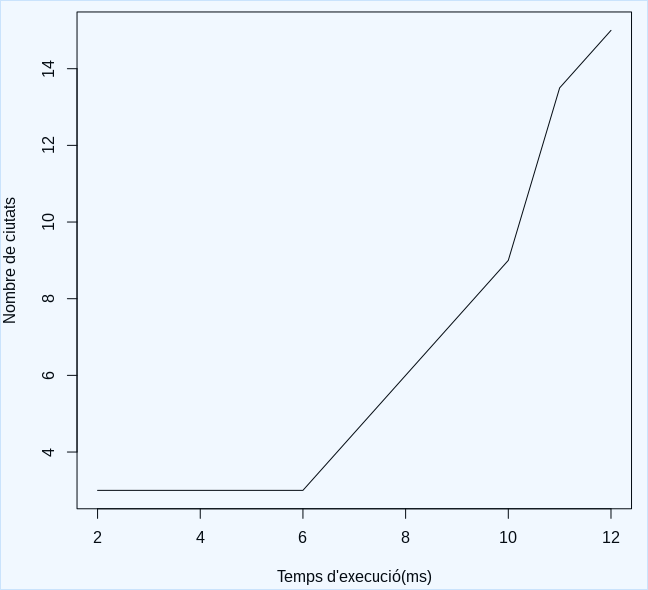
\includegraphics[width=\textwidth]{./grafic_experiment.png}
\caption{Temps d'execució de \emph{Metric-FF} en funció del nombre de ciutats del problema.}
\label{fig:grafic_experiment}
\end{figure}


\subsection{Conclusions}

Podem concloure que el resultat era l'esperat, s'ha obtingut un temps de mida creixent amb un comportament quadràtic per a problemes de mida creixent.

També cal comentar el fet que hem descobert un possible comportament \emph{greedy} per instàncies de mida prou petita, cosa que podria contradir en part el que ens havien comentat a classe de teoria sobre \emph{Fast Forward}\footnote{Tenim entès que Fast Forward no fa una aproximació voraç per problemes d'optimització. No obstant no hem comprovat aquest fet en el codi i ens basem únicament en els resultats empírics}. No obstant cal recordar que aquest programa és producte d'un concurs anual i que està en constant evolució, així que canvis d'aquest estil son d'esperar.

Per últim fa falta dir que desconeixem la causa del problema que ens ha impedit experimentar amb problemes de mida més gran que 12, cosa que hagués augmentat considerablement la validesa d'aquest experiment, però tal com hem comentat, el fet que sigui la mida del fitxer el que genera els errors apunta a que el problema es troba en el parser, i queda totalment fora de l'àmbit d'aquest treball el fet d'arreglar el solver.

\subsection{Replicabilitat}

Per tal d'assegurar la replicabilitat del nostre experiment, o ampliar-lo en cas que es disposi d'una versió arreglada de \emph{Metric-FF}, s'ha inclòs una carpeta \emph{Experiment} juntament amb aquesta entrega amb tots els scripts utilitzats. Des d'un entorn linux de 64 bits es pot repetir l'experiment executant els scripts \texttt{genera\_instancies.sh} i tot seguit \texttt{runner.sh}. 

Canviant l'executable de Metric-FF de la carpeta per un altre de compilat per la plataforma en qüestió aquest experiment s'hauria de poder replicar en qualsevol entorn \emph{Unix} amb un intèrpret de \emph{bash} (o fins i tot \emph{Windows} si es fa servir \emph{Cygwin}).

\end{document}